\documentclass[a4paper,12pt]{article}

% Paquetes
\usepackage[utf8]{inputenc}
\usepackage{graphicx}
\usepackage{amsmath, amssymb}
\usepackage[margin = 1in]{geometry}
\usepackage[spanish, es-tabla]{babel}
\spanishdecimal{.}
\usepackage{color}
\usepackage{hyperref}

\usepackage{inconsolata}
\usepackage{listings}
\usepackage{xcolor}

\lstset{
    language=C,
    basicstyle=\ttfamily\scriptsize,
    numbers=left,
    numberstyle=\tiny,
    numbersep=5pt,
    %backgroudcolor={gray!10},
    keywordstyle=\color{blue},
    commentstyle=\color{gray},
    stringstyle=\color{red},
    showstringspaces=false,
    frame=single,
    breaklines=true,
    tabsize=2,
    captionpos=t,
    extendedchars=true,
    literate={á}{{\'a}}1 {é}{{\'e}}1 {í}{{\'i}}1 {ó}{{\'o}}1 {ú}{{\'u}}1 {Ú}{{\'U}}1 {ñ}{{\~{n}}}1 {°}{{$^{\circ}$}}1
}

% Comandos
\newcommand{\R}{\mathbb{R}}
\newcommand{\Z}{\mathbb{Z}}
\newcommand{\N}{\mathbb{N}}
\newcommand{\var}{\operatorname{Var}}
\newcommand{\cov}{\operatorname{Cov}}
\newcommand{\E}{\mathbb{E}}
\newcommand{\norm}[1]{\left\Vert#1\right\Vert}

\renewcommand{\O}{\mathcal{O}}
\renewcommand{\P}{\mathbb{P}}

% Título
\title{Física computacional - Modelo de Ising \\ Laboratorio 4}
\author{El mono}
\date{}

% Documento
\begin{document}

\maketitle

\begin{abstract}
    Simulamos el modelo de Ising y calculamos algunas variables termodinámicas usando el método de Metropolis. Estudiamos la dependencia de estas variables con respecto a la temperatura del sistema y, en particular, observamos que existe una temperatura crítica $T_c$ en la cual la magnetización presenta una bifurcación. Esto es, una transición de fase.
\end{abstract}

\section{Introducción}

En este trabajo simulamos el modelo de Ising y calculamos algunas variables termodinámicas usando Markov Chain Monte Carlo (MCMC) con una cadena generada mediante el método Metropolis \cite{metropolis1953equation}. Concretamente, simulamos un toro discreto de $n^2$ partículas, cada una de las cuales puede tener spin {\it up} o {\it down}; y calculamos, en función de la temperatura $T^*$ (reducida) la magnetización $M$, la energía $E$, la susceptibilidad $\chi$, el calor específico $C$ y la temperatúra crítica $T_c$. Estos cálculos son, en general, de la forma
\begin{equation}
    \label{eq:ejemplo}
    Q = \E(f_Q(X)),
\end{equation}
donde $X : \Omega \to S$ es una variable aleatoria que cae en el espacio $S$ de esatados del sistema con distribución de Boltzmann, y $f_Q : S \to \R$ es alguna función por medio de la cual se calcula la cantidad $Q$.\\

Dado que el espacio de estados $S$  es de cardinal $2^{n^2}$ (pues cada una de las $n^2$ partículas puede tener spin {\it up} o {\it down}), es demasiado costoso calcular $Q$ por definición. Por esta razón usualmente se opta por aproximar $Q$ mediante integración Monte Carlo (MC). Sin embargo, no es trivial implementar este método de integración sobre $S$ (pensándolo como un espacio de probabilidad con la distribución de Boltzmann). Una cantidad considerable de teoría de probabilidades es necesaria para entender (al menos, superficielmente) por qué funciona esta técnica y cuáles son sus limitaciones. En la siguiente sección presentamos un poco de esta teoría (para más detalle, ver \cite{janke2009statistical,schachinger2007mcmc}).

\section{Preliminares}
\label{sec:preliminares}

En esta sección explicamos brevemente el método de Metrópolis y su utilidad en el contexto de la integración Monte Carlo. Esto es porque creemos que conocer ciertos detalles de la teoría de probabilidades puede ayudar a entender algunos de los fenómenos que se observan más adelante en las simulaciones numéricas.

\subsection{Monte Carlo Markov Chain}

Recordemos que la integración MC para calcular \eqref{eq:ejemplo} requiere una forma de muestrear $X$, esto es, una forma de generar una sucesión de estados que sean realizaciones de variables $X_n$ independientes e idénticamente distribuídas con la distribución de $X$. Hay varias formas de hacer esto, una de ellas consiste en generar una cadena de Markov tal que sus variables se aproximen a una muestra de $X$. De aquí el nombre: {\it Markov Chain Monte Carlo}.\\

Supongamos que existe una cadena de Markov $Y = (Y_n)$ sobre $S$ con una única distribución invariante $\pi$ igual a la distribución deseada (en este caso, la distribución de Boltzmann). Entonces, independientemente de la distribución inicial (generalmente $Y_0$ es uniforme o atómica), $Y_n$ converge debilmente\footnote{Esto es, $\E(h(Y_n)) \to \E(h(X))$ para toda $h$ continua y acotada.} a $X$. Así, a partir de cierto $N \in \N$, la cadena $Z = (Y_{N + n})$ se distribuye aproximadamente $\pi$. El fragmento restante de la cadena: $Y_0, Y_1, \dots, Y_{N - 1}$ se llama el {\it burn-in} y se descarta.

Ahora, si bien $Z$ es un proceso de Markov donde cada $Z_n$ se distribuye aproximadamente $\pi$, los $Z_n$ podrían no ser independientes (recordemos que estamos en busca de una muestra de $X$, para lo cual la independencia es un factor crucial). En estas circunstancias es necesario extender la teoría de integración MC al caso MCMC con muestreo no independiente y calcular nuevamente la varianza de la integral. En este trabajo no discutimos estos cálculos, simplemente mencionamos que la varianza de la integral MC es ahora inversamente proporcional al número de muestras (como antes) y proporcional a $\tau_a$, una variable llamada tiempo de autocorrelación que representa, intuitivamente, cuantas muestras $Z_n$ debemos descartar para emular un muestreo independiente. En otras palabras, $\tau_a$ se define de forma que el proceso
\begin{equation*}
    W = (Z_0, Z_{\tau_a}, Z_{2\tau_a}, \dots)
\end{equation*}
no presente evidencia de dependencia.\\

Sobre el final del trabajo estimaremos algunos tiempos de autocorrelación mediante la ecuación (ver \cite{janke2009statistical, schachinger2007mcmc})
\begin{equation}
    \label{eq:tiempo_de_autocorrelacion}
    \tau_a = \dfrac{1}{2} + \sum_{k \in \N} A(k),
\end{equation}
donde
\begin{equation}
    \label{eq:autocorrelacion}
    A(k) = \dfrac{\cov (f_Q(Z_0), f_Q(Z_k))}{\var (f_Q(Z_0))} = \dfrac{\E(f_Q(Z_0)f_Q(Z_k)) - \E^2(f_Q(Z_n))}{\E((f_Q(Z_0))^2) - \E^2(f_Q(Z_n))}
\end{equation}
es la función de autocorrelación del proceso $f_Q(Z)$ y depende de la variable termodinámica $Q$ que estemos estimando.

\subsection{Método de Matropolis}

Una forma ampliamente utilizada para construir una cadena de Markov con distribución invariante dada (en nuestro caso, la distribución de Boltzmann) es el método de Metropolis-Hastings. Este método define una cadena \( (Y_n) \) sobre el espacio de estados \( S \) a partir de una \emph{propuesta} de transición, esto es, una familia de distribuciones de probabilidad \( g(x' \mid x) \), que especifica la probabilidad de proponer un nuevo estado \( x' \in S \) dado el estado actual \( x \in S \).\footnote{Formalmanete, se especifica una familia de medidas de probabilidad indexadas por $S$, pero por consistencia con la bibliografía, denotamos esta familia por medio de sus funciones densidad condicional $g(\; \cdot \mid x)$ a pesar de que no necesariamente son absolutamente continuas con respecto a la medida de Lebesgue.} A partir del estado actual \( Y_n = x \), se genera un candidato \( x' \sim g(\; \cdot \mid x) \), el cual es aceptado con probabilidad
\begin{equation}
    \label{eq:p_aceptacion}
    \P(\text{aceptar } x' \mid x) = \min \left\{1, \frac{\pi(x')\, g(x \mid x')}{\pi(x)\, g(x' \mid x)} \right\},
\end{equation}
y rechazado (manteniendo el estado actual \( Y_{n+1} = x \)) con la probabilidad complementaria. Este procedimiento garantiza que la cadena resultante sea reversible con respecto a \( \pi \) y, bajo ciertas condiciones, ergódica. En particular, el método prouesto originalmente por Metropolis consideraba únicamente familias de distribuciones simétricas. Esto es, $g(x \mid x') = g(x' \mid x)$, de forma que la ecuación \eqref{eq:p_aceptacion} se simplifica.\\

Será importante notar el siguiente comportamiento en el método de Metropolis. Hemos dicho que a partir de un estado $Y_n = x$ se samplea (con distribución $g(\; \cdot \mid x)$) un nuevo punto, al que más tarde decidiremos si movernos o no (con probabilidad dada por \eqref{eq:p_aceptacion}). Intuitivamente, la sucesión $Y_n$ navega por $S$ pegando saltos de longitud dada por $g$. ¿Qué ocurre si la distribución invariante $\pi$ es, por poner un ejemplo, bimodal con dos regiones de alta probabilidad separadas por un valle de baja probabilidad? Si $g$ tiene poca varianza e $Y_n = x$ se encuentra en una de las regiones de alta probabilidad, es poco probable que {\it salte} hacia la otra region. Si bien está garantizado (por la convergencia debil) que eventualmente $Y_n$ saltará hacia la otra región, en un experimento numérico, esto puede demorar mucho. Es posible que al hacer MCMC con este tipo de distribuciones, la realización de $Y_n$ que usemos no represente $\pi$ (como queremos) sinó la restricción de $\pi$ a una de estas regiones.\\

En resumen, el método de Metropolis es una forma de generar una cadena de Markov con la cual se aproxima una muestra de una distribución $\pi$. Con esta muestra se calcula la integral MC. Entre las limitaciones más importantes de esta técnica tenemos que: debemos descartar el {\it burn in}, cuyo tamaño es desconocido y difícil de acotar eficientemente, no tenemos independencia, aunque podemos simularla conociendo $\tau_a$ (también, desconocido y difícil de acotar eficientemente), y ciertas distribuciones pueden ser difíciles de representar, si no se modifica la distribución de propuestas $g$. En particular, la distribución de Boltzmann en el espacio de estados del modelo de Ising tiene forma bimodal si $T$ es cercana a la temperatura crítica $T_c$, por lo que se necesitan muestreos extremadamente largos para obtener resultados confiables.

\section{Resultados}

En la Figura \ref{fig:a} presentamos, en función del número $N$ de pasos MC, los resultados de la integral MC de la magnetización $M$ y energía $E$ de un modelo de Ising de tamaño $40 \times 40$ con condiciones de borde periódicas. Por simplicidad, llamaremos $\langle M \rangle$ y $\langle E \rangle$ a los resultados de estas integrales. Hacemos gráficos diferentes para diferentes temperaturas, y comparamos los casos donde el primer estado tiene todos los espines {\it up} (llamado {\it cold start}, porque su baja energía) y donde el primer estado tiene espines aleatorios (llamado {\it hot start}).\footnote{Inciso a.}

\begin{figure}[h!]
    \centering
    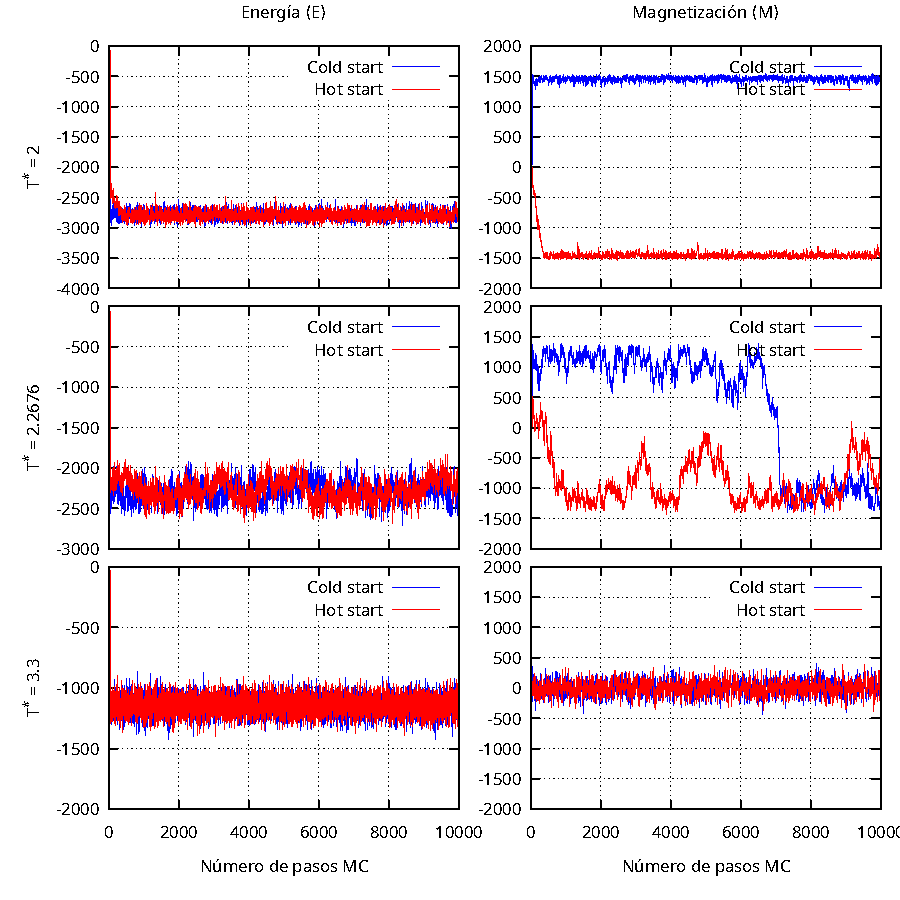
\includegraphics[width = \textwidth]{../img/a.pdf}
    \caption{Valores de $\langle M \rangle$ y $\langle E \rangle$ en función del número de pasos MC.}
    \label{fig:a}
\end{figure}

En la Figura \ref{fig:b} presentamos,\footnote{Inciso b.} como función de la temperatura reducida $T^*$, el valor absoluto de la magnetización por partícula, la energía por partícula, la susceptibilidad y el calor específico. Estimamos todos estos valores por integración MC con $N = 10000$ pasos y un {\it burn in} de 1000 pasos. Hacemos esto para modelos de Ising de tamaños $n = 10$, $n = 20$ y $n = 40$, donde $n$ es el número de partículas por lado. En la Figura \ref{fig:b_bis} presentamos, para discutir posteriormente, un acercamiento de los gráficos de la Figura \ref{fig:b}.

\begin{figure}[h!]
    \centering
    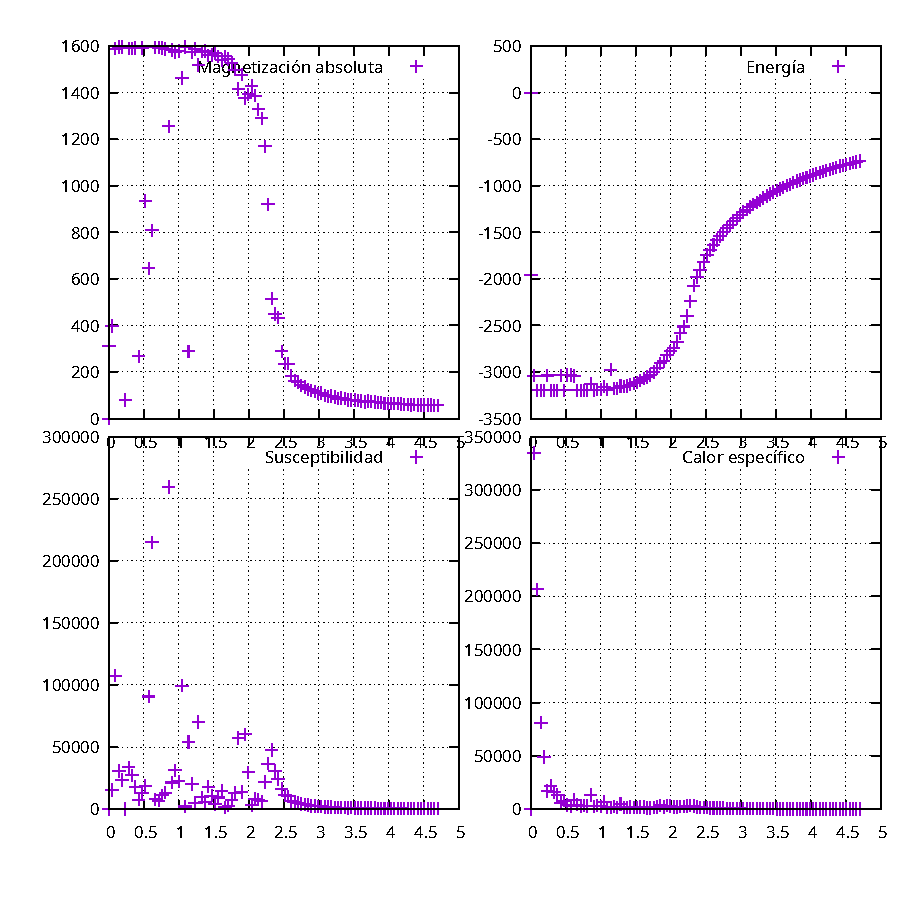
\includegraphics[width = .9\textwidth]{../img/b.pdf}
    \caption{Algunas variables termodinámicas en función de la temperatura reducida $T^*$.}
    \label{fig:b}
\end{figure}

\begin{figure}[h!]
    \centering
    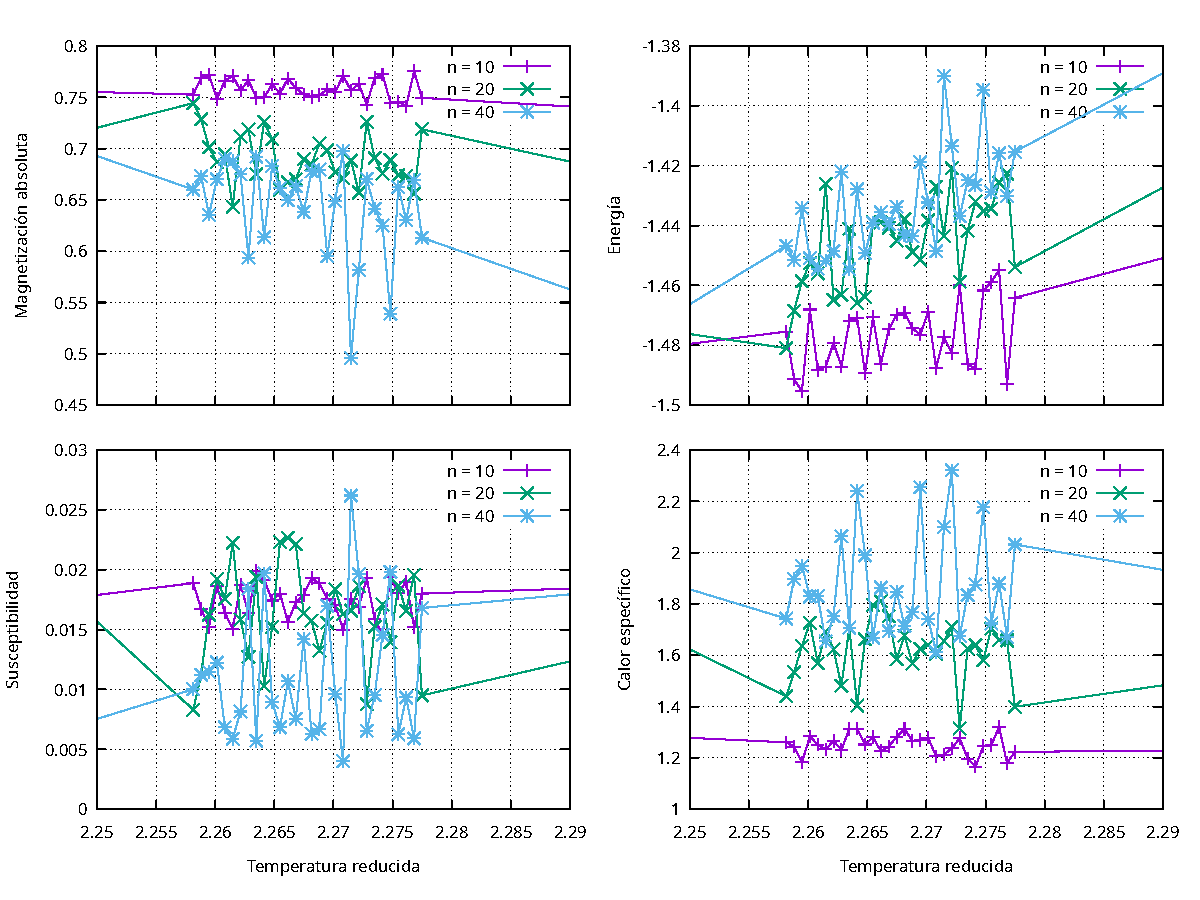
\includegraphics[width = .9\textwidth]{../img/b_bis.pdf}
    \caption{Acercamiento de la Figura \ref{fig:b}.}
    \label{fig:b_bis}
\end{figure}

\newpage

En la Figura \ref{fig:c} presentamos,\footnote{Inciso c.} para dos temperaturas reucidas diferentes (una ligeramente por encima y otra ligeramente por debajo de la temperatura crítica $T_c = 2.2676$), los histogramas de la magnetización en el modelo de Ising de tamaño $40 \times 40$. Para esto, como antes, excluímos un {\it burn in} de 1000 pasos MC y armamos el histograma con los datos de magnetización de $N = 10000$ estados del modelo.

\begin{figure}[h!]
    \centering
    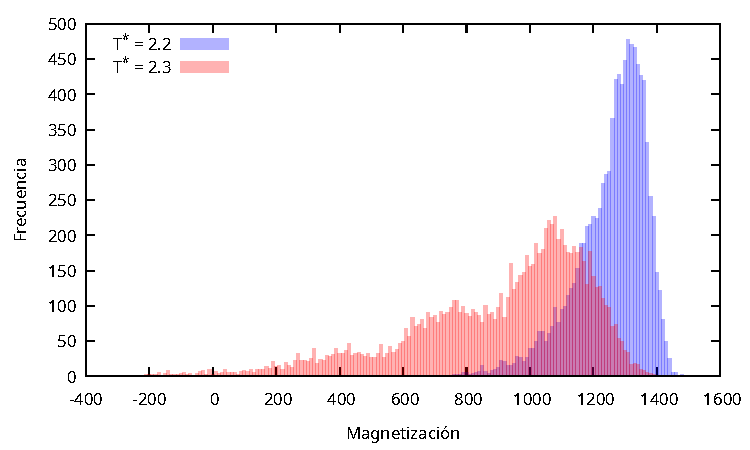
\includegraphics[width = .8\textwidth]{../img/c.pdf}
    \caption{Histogramas de $\langle M \rangle$ a diferentes temperaturas.}
    \label{fig:c}
\end{figure}

En la Figura \ref{fig:d} presentamos,\footnote{Indiso d.} para distintos tamaños de modelo, los {\it cumulantes de Binder}. Calculamos estos valores a partir de datos de magnetización obtenidos por integración MC con {\it burn in} de 1000 pasos y tamaño de muestra de $N = 100000$ pasos MC. Notese el incremente en el número de pasos.

\begin{figure}[h!]
    \centering
    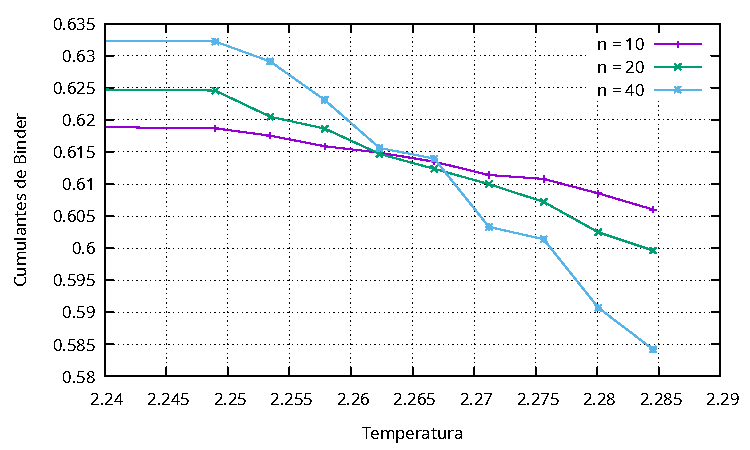
\includegraphics[width = .8\textwidth]{../img/d.pdf}
    \caption{Cumulantes de Binder para modelos de diferentes tamaños.}
    \label{fig:d}
\end{figure}

En la Figura \ref{fig:d_bis} mostramos los valores de $\langle |M| \rangle$ y $\chi$ obtenidos anteriormente por integración MC junto con las funciones $(T_c - T)^\beta$ y $|T - T_c|^{-\gamma}$. Se usan los exponentes críticos $\beta = \frac{1}{8}$ y $\gamma = \frac{7}{4}$ encontrados por Onsager [CITA A ONSAGER].

\begin{figure}[h!]
    \centering
    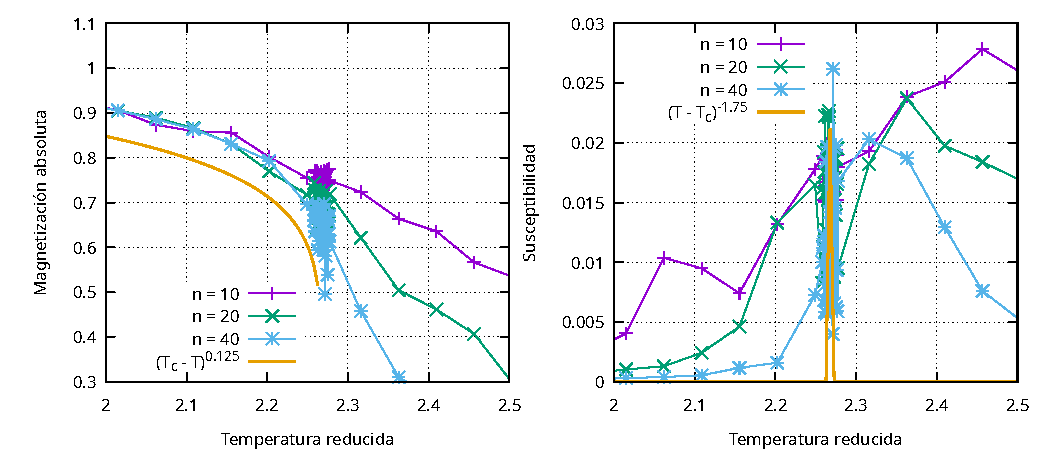
\includegraphics[width = \textwidth]{../img/d_bis.pdf}
    \caption{Exponentes críticos.}
    \label{fig:d_bis}
\end{figure}

Finalmente, en la Figura \ref{fig:e} presentamos las funciones de autocorrelación de la magnetización $|M|$ y energía $E$ calculadas a partir de los estados dados por el método de Metropolis. En función de estos datos, en la Tabla \ref{tab:tau} presentamos cotas para los tiempos de autocorrelación de magnetización $\tau_M$ y energía $\tau_E$.

\begin{figure}[h!]
    \centering
    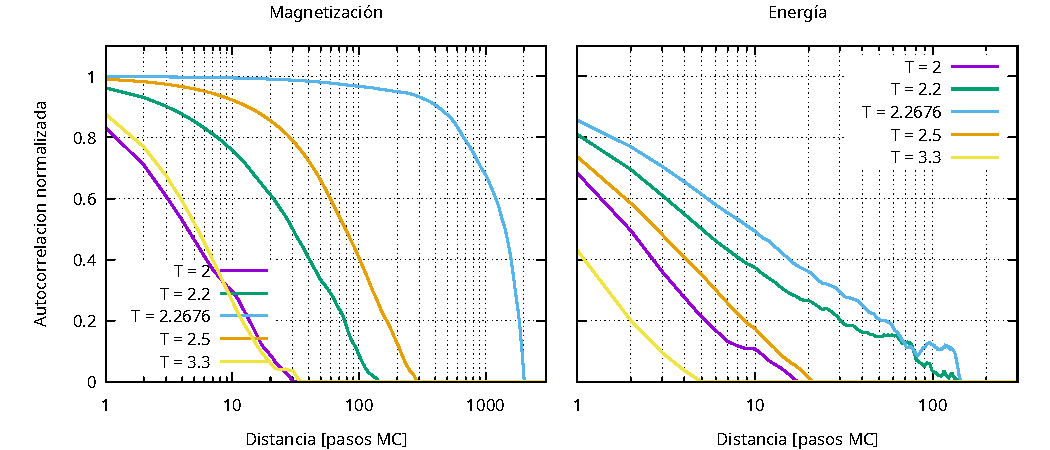
\includegraphics[width = \textwidth]{../img/e.pdf}
    \caption{Funciones de autocorrelación de $|M|$ y $E$.}
    \label{fig:e}
\end{figure}

\newpage

\begin{table}[h!]
    \centering
    \begin{tabular}{c|c|c}
        $T$ & $\tau_M$ & $\tau_E$ \\ \hline
        2 & 7.4 & 3.5 \\
        2.2 & 40.9 & 20.3 \\
        2.2676 & 1179 & 29.7 \\
        2.5 & 96 & 5  \\
        3.3 & 7.5 & 1.3  \\
    \end{tabular}
    \caption{Tiempos de autocorrelación \( \tau_M \) y \( \tau_E \) en función de $T$.}
    \label{tab:tau}
\end{table}

\section{Discusión}

Dividimos esta sección en varias subsecciones porque de otra forma sería muy extensa. Para este trabajo nos enfrentamos a muchas cosas nuevas y esto conlleva (inevitablemente) una discusión prolongada. La primera subsección es por lejos la mas importante, porque las consecuencias de las observaciones que se discuten en ella explican (en cierto sentido) las observaciones que se discuten en las demas subsecciones.

\subsection{Muestreo de $S$ con el método de Metropolis}

Intuitivamente, el muestreo por cadenas de Markov produce una sucesión distribuídos aproximadamente por la distribución de Boltzman. Esta distribución depende de la temperatura (reducida) $T^*$ y asigna probabilidades mas altas a estados de menor energía (ver \cite{phillies2000elementary}). Para temperaturas bajas (por debajo de $T_c$) el resultado de esto es que los sistemas muestreados tienden a tener espines alineados (ya sea {\it up} o {\it down}, el modelo de Ising es simétrico en este sentido). Para temperaturas altas (por encima de $T_c$) ocurre lo contratio: los sistemas muestreados tienden a tener espines aleatorios.\footnote{Estaría bueno tner peliculitas para mostrar de esto.} Dado que la magnetización depende de la suma de los espines (midiendo, en cierto sentido, la alineación general del sistema), es de esperarse que para temperaturas bajas, sea muy alta, y para temperaturas altas, sea cercana a 0. Esto es lo que se oberva en las gráficas del lado izquierdo de la Figura \ref{fig:a}. Por otro lado, la energía depende de (el negativo de) la suma de los productos de espines cercanos (midiendo, en cierto sentido, la alineación particular/local del sistema), así que es de esperarse que sea baja a temperaturas bajas y alta a temperaturas altas, como se observa en las gráficas del lado derecho de la Figura \ref{fig:a}.

Hamos mencionado en la Sección \ref{sec:preliminares} que el sampleo por cadenas de Markov produce un {\it burn in} que debe desecharse, esto se ve al inicio de las gráficas de la Figura \ref{fig:a}\footnote{O en el videíto si lo tuviéramos...} pero es más notorio a temperaturas bajas con un {\it hot start} (pues el estado inicial es desordenado y debe ordenarse) o temperaturas altas con un {\it cold start} (pues el estado inicial es ordenado y debe desordenarse). En la Figura \ref{fig:a_bis} mostramos un acercamiento de la Figura \ref{fig:a} en estos dos casos.

Sobre el final de la Sección \ref{sec:preliminares} mencionamos también que en distribuciones bimodales donde la probabilidad se concentra en regiones cercanas a las modas y separadas por valles de probabilidad baja, el muestreo por cadenas de Markov puede tardar mucho en producir una muestra aproximadamente independiente. Este es el caso de la distribución de Boltzman para el modelo de Ising a temperaturas por debajo de $T_c$. Esta es una observación sumamente interesante, porque al ver las gráficas de la Figura \ref{fig:a} correspondientes a $T^* = 2.2676$, uno podría sospechar que exhiben un comportamiento no deseado, y que debería ocurrir algo como lo que ocurre en las gráficas correspondientes a $T^* = 2$. Sin embargo, es todo lo contrario. Los datos de magnetización en $T^*"= 2$ muestran que la cadena de Markov con la cual sampleamos los estados para la integración MC se estancan: el {\it cold start} se implementó como el estado con todos los espines {\it up}, y la cadena de Markov generada a partir de este estado se estancó allí, produciendo una sucesión de estados similares, mientras que en realidad, los estados generalmente alineados {\it up} son igual de probables que los estados generalmente alineados {\it down}. De manera similar, el {\it hot start} dió lugar a una cadena de estados que terminan alineandose mayoritariamente {\it down} (aunque podrían haber sido {\it up}) y se estancan allí.

Las gráficas correspondientes a $T^* = 2.2676$, en cambio, exhiben un comportamiento mas deseable. Si bien las cadenas de Markov que generan los estados se estancan en regiones cercanas a una de las modas, eventualmente son capaces de saltar a la región cercana a la otra moda. Esto nos dice que para $T_c$, a pesar de que la distribución de Boltzman del modelo de Ising es bimodal, las regiones de alta probabilidad cercanas a cada moda estan relativamente cerca. Al menos, suficiente para que la distribución de la propuesta de salto $g(\; \cdot \mid x)$ pueda saltar de una a otra.

Esta observación nos conduce a una sugerencia para evitar el problema: cambiar la distribución de $g$. En nuestro caso, la probabilidad $g(\; \cdot \mid x)$ es uniforme sobre el conjunto $X = \{x' \in S : d_H(x', x) = 1 \}$. Esto hace extremadamente improbable que la cadena de Markov pueda saltar de la región cercana a una moda hasta la región cercan a la otra moda cuando la temperatura es baja. Un algoritmo diferente, como por ejemplo, proponer varios flips simultaneos y {\it luego} calcular $\Delta E$, representaría una distribución $g$ mas amplia, por lo que podría ayudar a muestrear mejor la distribucioń de Boltzmann en temperaturas cercanas a $T_c$. Por supuesto, esto no soluciona el problema, simplemente lo desplaza. Ahora el fenómeno que dificulta el sampleo, en lugar de presentarse en $T_c$, se presentaría en alguna otra temperatura menor a $T_c$.

Para para para para, entonces justo el algoritmo de sampleo qu enos dieron falla JUSTOen la temperatura que queremos estudiar? Si

Ahora, si esto es correcto, significa que una distribución para la propuesta de salto diferente podría resolver estos problemas, o tendría problemas en otras regiones. No? Deberíamos proopner otra distribución para la propuesta de salto y testearla. Aunque en en realidad primero debería discutirlo con Guidex para asegurarme de que entendí bien las cosas.

La Figura \ref{fig:a} tiene todavía una característica más, digna de observación. en t bajas, ocurre que tenemos bimodalidad

Recordemos que enEn temperaturas por debajo de la crítica, recordemos que la distribución de probabilidad es (intuitivamente) bimodal, donde ambas modas son los estados donde los espines estan completamente alineados (todos {\it up} o todos {\it down}). Por lo mencionado sobre el final de la Sección \ref{sec:preliminares}, es de esperarse que los estados sampleados oscilen entre las dos 

Aca ponemos comentarios sobre el inciso a, que justamente nos dice que tan estable es el muestreo. Y de donde estimamos que un burn in de 1000 puntos es razonable para la mayoría de las temperaturas (ya cerca de $T_c$ no hay nada que hacer...).

\subsection{Variables termodinámicas}

Pasamos ahora al inciso 2, lo importante es notar que todo parece en orden salvo cerca de las temperaturas críticas, esto va a ser un factor común en todos los resultados (salvo los relacionados con los cumulantes de Binder, que son un poco mas estables). Pusimos un zoom in de esttos graficos justamente para que se aprecie.

Analizamos tambien los histogramas aca, que estan indicando que la magnetización a temperaturas por encima de la crítica es desorganizada (lo cual es esperable) y temperaturas por debajo de la crítica son estables y se agrupan.

\subsection{Estimación de $T_c$}

Para esto existen los cumulantes de Binder, no se suficiente física así que no voy a emitir comentario al respecto. Aca es donde digo que tiene pinta que algo pasa entre 2.2625 y 2.2675. Sin embargo mi compu tiro corridas de $N = 100000$ y no dio para mas, así que hasta ahí llega nuestra precision.

\subsection{Autocorrelación y estimación de errores}

Como mencionamos en la sección \ref{sec:preliminares}, la varianza de la integración monte carlo en casos de muestreo no independiente es mayor que la de muestreo independiente. Se estima mayor en un factor $\tau_a$, que estimamos en la Table \ref{tab:tau}, así que a pesar de que usamos $N = 10000$, con lo cual deberíamos esperar resultados con desviación de 0.01 unidades, la verdadera desviación debe multiplicarse por $\sqrt{\tau_a}$.

Por poner un ejemplo, en la Figura \ref{fig:c} vemos que la magnetización con $N = 10000$ tiene media 0 y hemos calculado que tiene varianza 1.19e5. O sea una desviación de 345 mas o menos. La desviación si todo fuera independiente es 0.01 multiplicado por los valores de la variable que se estan tomando, que ronda los 1600 diría yo, entonces esperamos una desviación de 16 unidades... pero vemos una de 345! Ahora, la tabla nos dice que el $\tau_M$ para $T = 2.5$ es de mas o menos 96! que tiene raiz mas o menos 10, lo cual nos lleva de 16 unidades de desviación a 160 mas o menos, mucho mas cerca de las 345 observadas experimentalmente. Este es un ejemplo de mierda, por supuesto, ojala pudiéramos hacer otro. De hecho, podemos.

Mentira, no podemos poner ningun ejemplo porque precisamos conocer justamente la desviación de la propia función de energía o magnetización en el espacio de estados con la verdadera distribución de Boltzman! Si pudieramos estimar eso, entonces tendríamos como para laburar un buen ejemplo de la desviación esperada... pero bueno, no quiero hacerlo. No estaría mal ponerlo como si pudieramos intentarlo en el futuro.

\subsection{Cosas que me quedan por agregar.}

A medida que aumenta $n$, sabemos que la magnetización aleatoria se pelea con la temperatura. Si la temperatura $T^*$ es suficientemente grande, la probabilidad de aceptar un cambio crece, lo que conlleva mayor variabilidad de la magnetización en cada paso MC. Entonces, para temperaturas bajas, esperamos ver, en los {\it cold starts} que la magnetizacion general se mantiene, pues es poco propenso que el sistema acepte los cambios propuestos en un paso MC. Y en el {\it hot start}, esperamos ver uqe el sistema se decida rapidamente por una magnetización mas o menos uniforme y permanezca ahi. Esto es lo que se ve en los gráficos. Por mera casualidad, el hot start decidio estabilizarse con espin negativo...

Con respecto valores grandes de $T^*$ esperamos que la magnetización sea completamente aleatoria a lo largo de los pasos MC, pues se aceptan casi todos los cambios, sin importar si empezamos frios o calientes.

Lo interesante pasa para temperaturas intermedias. En $T^* = 2.2676$ observamos que la energía no se estabiliza, sinó que oscila (de forma no periódica) en un rango de enrgías. Al mismo tiempo, la magnetización tampoco se estabiliza, sinó que oscila entre períodos de magnetización casi uniformemente positiva y casi uniformemente negativa. Notemos ademas, que parecen coincidir los valores de $n$ para los cuales $\langle M \rangle$ oscila y $\langle E \rangle$ toma valores grandes. Esto nos indica que la distribución de Boltzmann para este valor de $T^*$ es (hablando mal y pronto) bimodal, y la cadena de Markov del método de Metropolis debe pasar un tiempo en la región dominada por una de las modas y otro tiempo en la región dominada por la otra moda. A medida que la cadena transiciona entre ambas regiones, pasa por estados de energía mas alta, por esto las transiciones en $\langle M \rangle$ se corresponden con incrementos en $\langle E \rangle$.

Uno podría pensar que en este caso la integral MC no converge rápidamente, por lo que habría utilizar algún método alternativo, una cadena de Markov distinta quizas, o cualquier otra alternativa. Sin embargo, en la opinión del autor, el hecho de que $\langle M \rangle$ no converge es evidencia de que estamos haciendo la pregunta incorrecta, no de que somos incapaces de responderla. Me explico: si sabes que tu distribución es bimodal, qué sentido tiene preguntarte por la media? No es información representativa de la distribución. La integral MC calcula correctamente la media (si es cierto que tarda bastante mas en converger), pero preguntarse por la media en una bimodal es inútil. De hecho, en el caso $T^* = 0$ la distribución de Boltzmann también es bimodal pero la integral de MC se estabiliza en una de las modas: ESTE ES EL VERDADERO ERROR! La verdadera integral de $M$ debería icluír información de ambas modas y equilibrarse en $\langle M \rangle = 0$. La falencia aquí es de la cadena de Markov del método de Metropolis, que no recorre correctamente el espacio de estados.

En principio, esto significa que no podemos confiar en los resultados calculados para temperaturas bajas! Sin embargo, dado que el sistema es simétrico con respecto al cambio de espines, aún podemos obtener resultados que ilustren el comportamiento del sistema si usamos el valor absoluto de la magnetización en lugar de la magnetización con signo. Repito: no cambiamos de $M$ a $|M|$ porque las cosas {\it se terminan promediando en 0} sino justamente porque no lo hacen. El problema es mas serio que simplemente no obtener información! ESTO TAMBIEN PODRÍA FRASEARSE COMO QUE ESTAMOS CAMBIANDO LA PREGUNTA.\\

Bueno, con respecto a los demas graficos no hay mucho que decir porque yo mismo no se mucho sober lo que esta pasando, puedo interpretar las probabilidades y demas cosas, pero no tanto la física. O decir a que corresponde macroscópicamente.... así que estas partes del informe van a quedar cortiñas... jaja willie cortiñas.

\section{Trabajo actual}

Todavía nos queda estimar bien $T_c$, aclara que no estamos tomando los burn-ins, y una vez que tengamos $T_c$ estimada, tenemos que aproximar los exponentes críticos usando regresión exponencial y presentar gráficos de eso, diría yo... aunque podemos cargarlo en los mismos gráficos que ya venimos teniendo, porque estan todos exponenciales...

Al discutir el error va a haber qu ecitar tanto el libro que me paso Guido que hay que rastrear como el paper de Jankel que nos paso la vero.

Disminuír cantidad de puntos y hacer simulaciones mas largas. La variabilidad parece aumentar con $n = 40$, eso podría ser porque a tamaños mas grandes, cuesta mas saltar entre las 2 modas de una distribución bimodal. Escribir eso... no se si tendremos tiempo para hacer una corrida mas larga para los experimentos. Sería mejor poner un poco de esfuerzo para estudiar lo que es el tema siguiente.


\section{Trabajo futuro}

\cite{phillies2000elementary} fue de mucha ayuda...

%Podríamos chusmear tambien https://archive.org/details/springer_10.1007-978-1-4757-4145-2/page/n15/mode/2up

Para este trabajo no fueron tantas las herramientas computacionales las que aprendimos sino mas bien las físicas. Estudiamos un poco de mecanica estadística para saber que estaba pasando, y estudiamos un montón de estadística para entender mas los procesos aleatorios y sus cearacterizaciones, como se prueban independencias y demas cosas. Es un trabajo agotador pero nuevamente, me encanta.\\

Otra vez podríamos haber usado CUDA pero no lo hicimos (aunque ya las cosas estaban tardando un pelin mas...).


ESTA ES LA ÚLTIMA SECCIÓN DE TRABAJO FUTURO, LA DEJO PARA TENER UNA REFERENCIA PARA ACTUALIZAR MAS TARDE.

Finalmente! Las imágenes tienen letra grande. Este es el más notorio de nuestros avances, pero hubo otros: adoptamos una estructura de carpetas {\it estandar} (en cierto sentido) para el código correspondiente a los ejercicios, automatizamos la compilación, testeo y generación de imágenes por medio de archivos \verb|makefile|, agregamos control de versiones por medio de Git y almacenamos el código en un repositorio online con GitHub. También estudiamos lo básico de CUDA, un lenguaje similar a C++ desarrollado por NVidia que permite programar para los procesadores de las GPUs, pero como los ejercicio de este laboratorio no eran demasiado costosos computacionalmente, no fue necesario implementar los generadores en este lenguaje. Esperamos, sin embargo, que cobre relevancia en laboratorios futuros.\\

Este ha sido, hasta el momento, el laboratorio más divertido. Entre las cosas que quedan por explorar, las más importantes son: el manual del compilador (opciones de optimización, tratar advertencias como errores, usar varios compiladores para detectar diferentes errores, etc), el lenguaje de scripting Bash, y temas básicos de mecánica estadística, para poder hacer los siguientes laboratorios.

%\section{Código}
%\label{sec:codice}
%\lstinputlisting[caption={Módulo con funciones auxiliares.}, label={lst:calor.c}]{../ej1/calor.c}

\bibliographystyle{abbrv}
\bibliography{biblio}

\end{document}